\documentclass[prd,showpacs,amsfonts,amssymb,amsmath, nofootinbib]{revtex4-1}

\usepackage{graphicx}
\usepackage{simplewick}
\usepackage{epstopdf}
\usepackage{multirow}
\usepackage{dcolumn}
\usepackage{hyperref}
\usepackage{cases}
\usepackage{bm}
\usepackage{epsfig}
\usepackage{color}
\usepackage[normalem]{ulem}
\usepackage{subfig}

\bibliographystyle{fapj}

\newcommand{\no}{\nonumber}

\def\be{\begin{equation}}
\def\ee{\end{equation}}
\def\bea{\begin{eqnarray}}
\def\eea{\end{eqnarray}}

\newcommand{\ha}{{1 \over 2}}
\newcommand{\la}{\lambda}
\newcommand{\rc}{\nonumber\\}

\newcommand{\bear}{\begin{eqnarray}}

\newcommand{\eear}{\end{eqnarray}}
\newcommand{\de}{\partial}
\newcommand{\tableskip}{\tablevspace{3pt}}
\newlength{\tskip}\setlength{\tskip}{5pt}
\newbox\pippobox

\def\be{\begin{equation}}
\def\ee{\end{equation}}
\def\bea{\begin{eqnarray}}
\def\eea{\end{eqnarray}}

\newcommand{\nver}{\hat{\mathbf{n}}}
\newcommand{\kver}{\hat{\mathbf{k}}}


\begin{document}

 
\title{Notes}

\author{Federico Bianchini$^{1,2}$, Andrew Jaffe$^{3}$}
\affiliation{
\smallskip
$^{1}$ SISSA - International School for Advanced Studies, Via Bonomea 265, 34136, Trieste, Italy \\
\smallskip
$^{2}$ INFN, Sezione di Trieste, Via Valerio 2, I-34127 Trieste, Italy\\
$^{3}$ Imperial Centre for Inference and Cosmology, Department of Physics, Imperial College London, Blackett Laboratory, Prince Consort Road, London SW7 2AZ, UK\\
\smallskip }


\begin{abstract}
In this notes, we review the CMB lensing - galaxy cross-correlation theoretical background and investigate  the impact of the redshift distribution modeling on the inferred theory parameters (i.e. linear galaxy bias $b$ and cross-correlation amplitude $A$). To this end, we first develop a spectral energy distribution (SED) template fitting machinery based on Bayesian formalism and recover full photometric redshift (photo-z) information about the Herschel-ATLAS galaxy sample considered here. Different photo-z estimates are used to model redshift distributions and predict theoretical lines which are then compared with data.
 
\end{abstract}

%\pacs{04.60.-m; 98.80.-k; 98.80.Bp; 98.80.Cq; 98.80.Qc}

\maketitle


\section{Theory}
\label{sec:theory}

Both the CMB convergence field $\kappa$ and galaxy density fluctuations $g$ along the line-of-sight (LOS) can be written as a weighted integral of the dark matter density contrast $\delta$ over the redshift:

\begin{equation}
X(\nver) = \int_0^{z_*} dz\, W^X(z)\delta(\chi(z)\nver,z),
\end{equation}

where $X=\{\kappa,g\}$ and $W^X(z)$ is the kernel related to a given field.
The kernel $W^{\kappa}$ describes the matter distribution lensing efficiency and it reads as follows
%
\begin{equation}
W^{\kappa}(z) = \frac{3\Omega_m}{2c}\frac{H_0^2}{H(z)}(1+z)\chi(z)\frac{\chi_*-\chi(z)}{\chi_*}.
\end{equation}
%
Here, $\chi(z)$ is the comoving distance to redshift $z$, $\chi_*$ is the comoving distance to the last scattering surface at $z_*\simeq 1090$, $H(z)$ is the Hubble factor at redshift $z$, $c$ is the speed of light, $\Omega_m$ and $H_0$ are the present-day values of matter density and Hubble parameter respectively.

Assuming that luminous matter traces the peaks of the dark matter distribution, the galaxy kernel is given by the sum of two terms:
%
\begin{equation}
W^{g}(z) = b(z)\frac{dN}{dz} + \mu(z).
\label{eqn:wg}
\end{equation}
%
The former is related to the intrinsic physical clustering of sources
and is directly proportional to the product between the bias\footnote{Throughout the analysis we assume a linear, local,
  deterministic, redshift- and scale-independent bias unless otherwise
  stated.}
$b$ and the \emph{unit-normalized} source redshift distribution $dN/dz$, while the
latter describes the effect of lensing magnification bias
\citep{turner84,villumsen95,xia09} and reads as follows:
%
\begin{equation}
\label{eqn:wmu}
\mu(z) = \frac{3\Omega_{\rm m}}{2c}\frac{H_0^2}{H(z)}(1+z)\chi(z) \int_z^{z_*}dz'\,\Bigl(1-\frac{\chi(z)}{\chi(z')}\Bigr)(\alpha(z')-1)\frac{dN}{dz}.
\end{equation}
%
This term is independent of the
tracers bias and, in the weak lensing limit, depends on the
logarithmic slope of the number counts $\alpha$ ($N(>F)\propto
F^{-\alpha}$) at the survey limiting magnitude.  \cite{gonzalez-nuevo:2014} has shown that the magnification bias by weak lensing is substantial for high-z H-ATLAS sources selected with the same criteria as the present sample. In this analysis the value is measured from the data and fixed to a fiducial value
$\alpha=3$.\\
The theoretical CMB convergence-galaxy angular cross-power spectrum and the galaxy auto-power spectrum can then be evaluated in the Limber approximation \citep{limber} as a weighted integral of the matter power spectrum $P(k,z)$:
%
\begin{equation}
\begin{split}
C_{\ell}^{\kappa g} &=   \int_0^{z_*} \frac{dz}{c} \frac{H(z)}{\chi^2(z)} W^{\kappa}(z)W^{g}(z)P(k=\ell/\chi(z),z); \\
C_{\ell}^{gg} &=   \int_0^{z_*} \frac{dz}{c} \frac{H(z)}{\chi^2(z)} [W^{g}(z)]^2P(k=\ell/\chi(z),z).
\end{split}
\end{equation}
%
We compute the non-linear $P(k,z)$ using CAMB\footnote{\url{http://cosmologist.info/camb/}} code with Halofit prescription \citep{camb,halofit}. \\


\section{Photo-z estimation}
\label{sec:photoz}
Photo-z estimations methods can be divided into two main approaches: the \emph{SED fitting} and the \emph{empirical training set}. Here, we shall focus on the former. The basic idea is to calculate the probability of a galaxy with observed fluxes $\mathbf{d}=\{ F_j\}$ (with $j$ labeling the photometry band) having a redshift $z$, \emph{assuming} that the galaxy SED is given by the template $T$. Bayes theorem tells us that
\be
\label{bayes_photoz}
p(\boldsymbol{\theta}| \mathbf{d},T) = \frac{p(\mathbf{d}| \boldsymbol{\theta},T)p(\boldsymbol{\theta}| T)}{p(\mathbf{d}|T)} \propto p(\mathbf{d}| \boldsymbol{\theta},T)p(\boldsymbol{\theta}| T),
\ee
where $\boldsymbol{\theta}=\{z,a\}$ is the model parameters vector. The expression $p(\mathbf{d}| \boldsymbol{\theta},T) = \mathcal{L}$ is the likelihood, giving the probability of observing fluxes $\mathbf{d}$ if the galaxy has redshift $z$ (and template normalization $a$):
\be
\label{like_photoz}
-2\log\mathcal{L} \propto \chi^2(z,a,T) = \sum_{\lambda} \biggl(\frac{F^{\rm obs}_{\lambda}-aF^{\rm th}_{\lambda}(z,T)}{\sigma_{\lambda}} \biggr)^2,
\ee
where $\sigma_{\lambda}$ are the uncertainties on the measured fluxes $F^{\rm obs}_{\lambda}$ and summation is extended on all observed bands. Theoretical fluxes are $F^{\rm th}_{\lambda}(z,T) \propto T(\lambda^{\rm obs}/(1+z))$, hence all other scalings in $z$ due to luminosity distance are incorporated in the SED template amplitude $a$ which we marginalize over. The other terms, $p(\boldsymbol{\theta}| T)$ and $p(\mathbf{d}|T)$, are the prior and the evidence (which is a normalization that we do not calculate). \\
In the present analysis, we make use of a single SED template, namely the one of SMM-J2135 which is shown in Fig.~\ref{fig:sed}. The presence of the \emph{shifting} peak in the frequency range covered by Herschel observation makes it suitable for photo-z estimation.

\begin{figure*}[!th]
\begin{center}
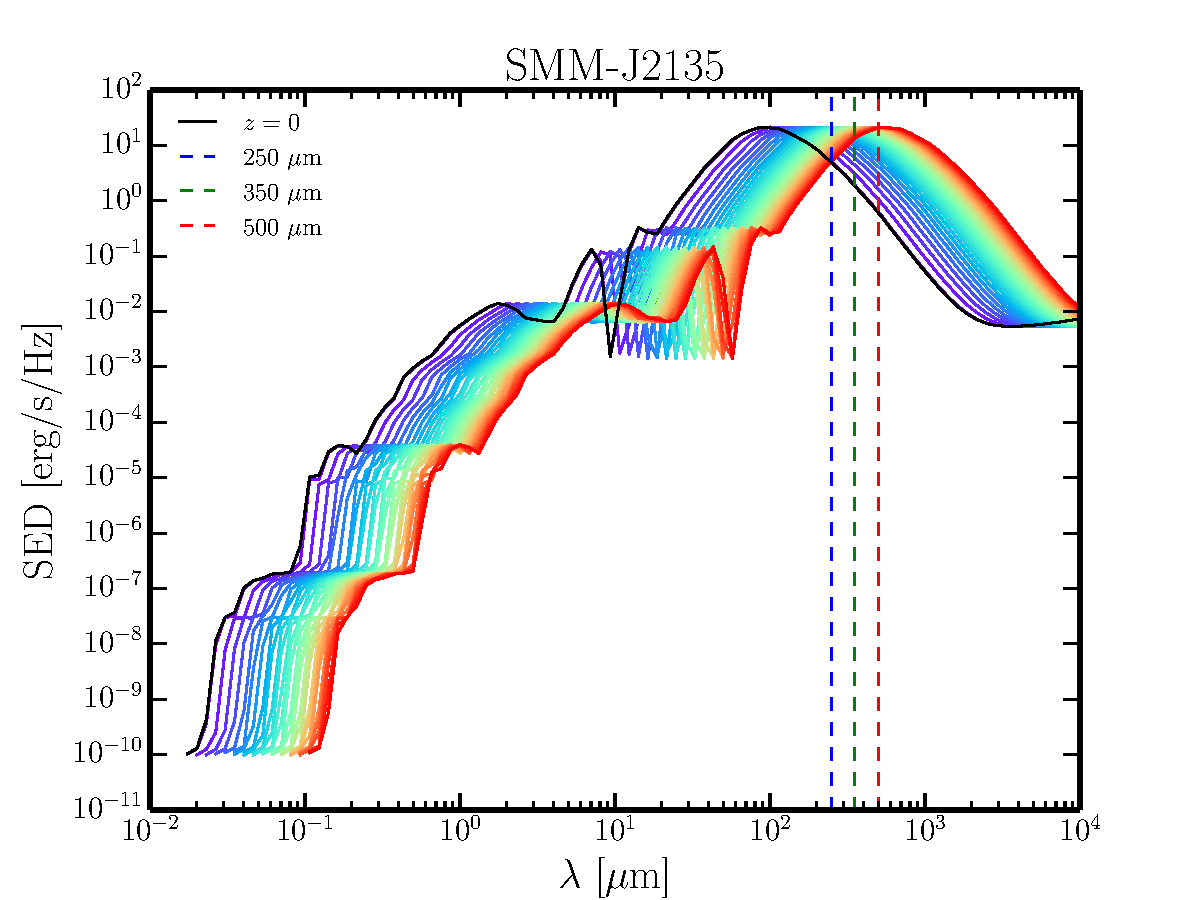
\includegraphics[width=0.8\textwidth]{images/SED_zs}
\caption{SED distribution template of SMM at $z=0$ (black solid line): solid colored lines from bluish to reddish represent rest-frame SED redshifted in the range $0 < z \le 5$. Colored dashed lines mark the wavelengths observed by the SPIRE instrument on Herschel.} 
\label{fig:sed}
\end{center}
\end{figure*}

We consider galaxies in the H-ATLAS fields (NGP+SGP+GAMA fields) which satisfy (i) the flux at 250 $\mu m$ $S_{250}> 35$ mJy; (ii) $3\sigma$ detection of the source galaxy at 350 $\mu$m. Then we exploit the observed fluxes and their associated errors at $\lambda=250,350,500$ $\mu$m, together with the SED, to sample the posterior in Eq.~\ref{bayes_photoz}. The parameter space is explored using emcee\footnote{\url{http://dan.iel.fm/emcee}}, an affine invariant Markov Chain Monte Carlo (MCMC) sampler \citep{emcee}, assuming flat priors over the range $\{z\} = \{[0,10]\}$ and Jeffreys priors over $\{a\} = \{[0,\infty)\}$. We then marginalize over the template amplitude parameter $a$ and obtain the posterior $p(z|\mathbf{d},T)$ for each one of the galaxy. An example of the outputs of this analysis step is shown in Fig.~\ref{fig:photoz_output}


\begin{figure}
\centering
\subfloat[Observed fluxes $F^{\rm obs}_j$ overimposed to the best-fit SED]{
  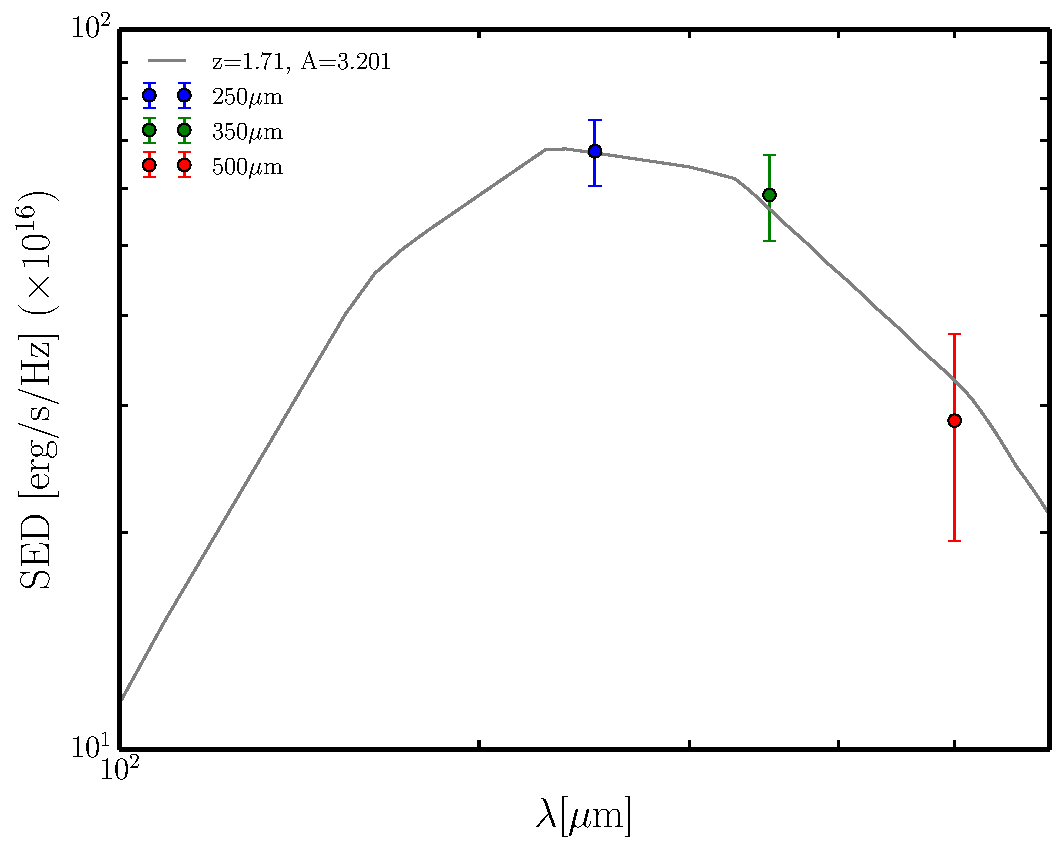
\includegraphics[width=65mm]{images/ex_fluxes}
}
\subfloat[Chains showing the position of the parameter space walkers as function of the iteration step. Burn-in phase removed before plotting.]{
  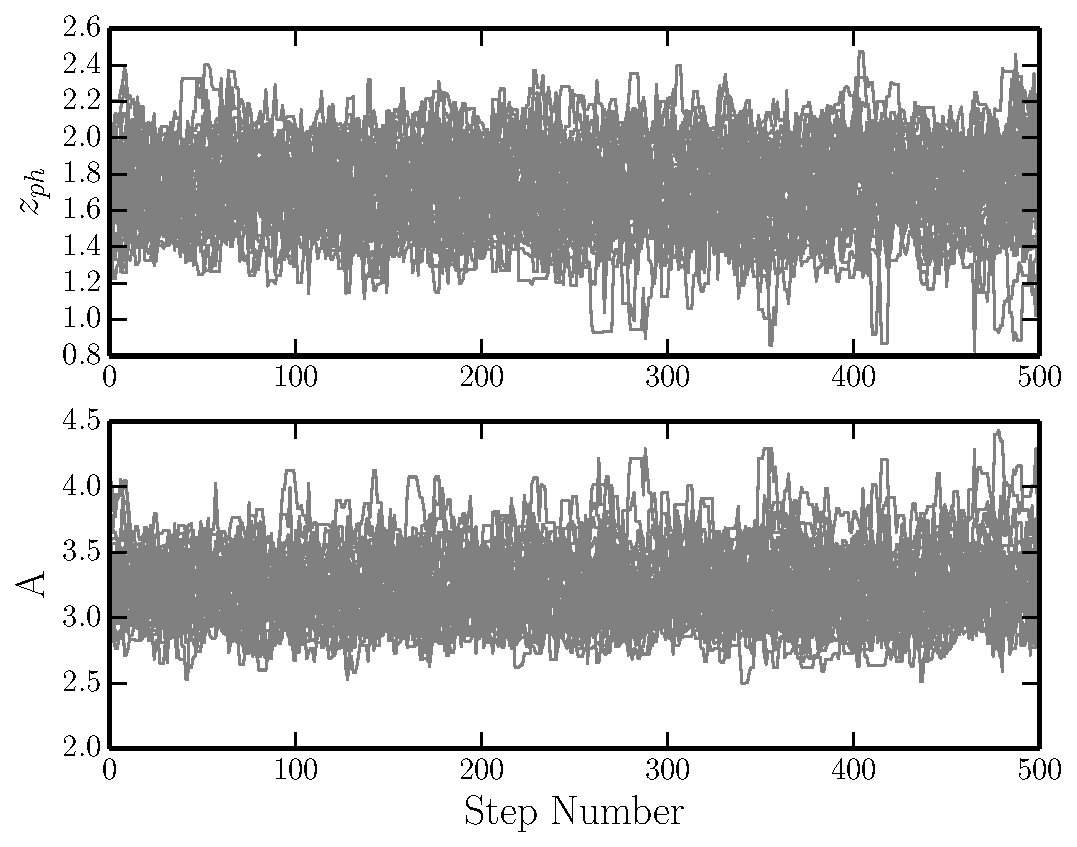
\includegraphics[width=65mm]{images/ex_chains}
}
\hspace{0mm}
\subfloat[Triangle plot showing 1 and 2$\sigma$ credible regions in the $z_{\rm ph}-a$ plane.]{
  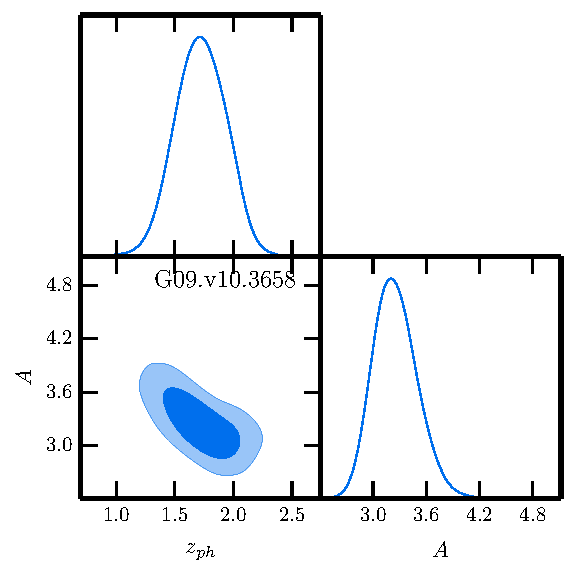
\includegraphics[width=65mm]{images/ex_triangle}
}
\subfloat[Posterior distribution $p(z|\mathbf{d},T)$ marginalized over $a$. Red dashed line highlights our best-fit (posterior peak) photo-z estimate, while the one provided by Joaquin Gonzalez-Nuevo is shown in grey.]{
  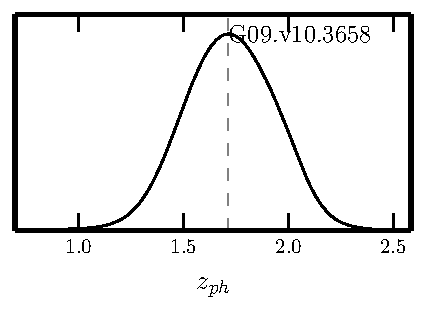
\includegraphics[width=65mm]{images/ex_1d}
}

\caption{An example of the plots output by the photo-z code relative to the G09.v10.3658 source.}
\label{fig:photoz_output}
\end{figure}

\section{Redshift distribution modeling}



\section{Estimation of cross-correlation amplitude and galaxy bias}

Following B15, we introduce a phenomenologically-motivated amplitude parameter $A$ that globally scales the observed cross-power spectrum with respect to the theoretical one as $\hat{C}^{\kappa g}_{L}=AC^{\kappa g}_{L}(b)$, where hat quantities refers to observed one and $L$ is the bandpower index  (hereafter $C^{XY}_{L}$ denotes the binned power spectrum and  $L$ identifies the bin).
We analyze the constraints on theory parameters by combining the cross- and galaxy auto-spectra information. For the joint analysis we exploit Gaussian likelihood functions that take into account correlations between the cross- and the autopower spectra in the covariance matrix. Extracted cross- and auto-bandpowers are organized into a single data vector as
%
\begin{equation}
\mathbf{\hat{C}}_{L} = (\mathbf{\hat{C}}^{\kappa g}_{L}, \mathbf{\hat{C}}^{gg}_{L}),
\end{equation}
%
which has $N_L=14$ elements. The total covariance matrix is then written as the composition of four $7\times7$ submatrices:
%
\begin{equation}
\textbf{Cov}_{LL'} =
\begin{bmatrix}
\text{Cov}^{\kappa g}_{LL'} & (\text{Cov}^{\kappa g-gg}_{LL'})^\intercal \\
 \text{Cov}^{\kappa g-gg}_{LL'} & \text{Cov}^{gg}_{LL'}  \\
\end{bmatrix}.
\end{equation}
%
The different covariance matrices are given by: 
%
\begin{equation}
\label{eqn:covs}
\begin{split}
{\text{Cov}}^{gg}_{LL'} &= \frac{2}{(2L+1)\Delta L f_{\rm sky}}\Bigl[C_{L}^{gg}(\boldsymbol{\theta}) + N_{L}^{gg}\Bigr]^2\delta_{LL'}
; \\
{\text{Cov}}^{\kappa g}_{LL'} &= \frac{1}{(2L+1)\Delta L f_{\rm sky}} \\ 
&\times\Bigl[(C_{L}^{\kappa g}(\boldsymbol{\theta}))^2 + (C_{L}^{\kappa\kappa} + N_{L}^{\kappa\kappa})(C_{L}^{gg}(\boldsymbol{\theta}) + N_{L}^{gg})\Bigr] \delta_{LL'} ; \\
{\text{Cov}}^{\kappa g-gg}_{LL'} &= \frac{2}{(2L+1)\Delta L f_{\rm sky}} \Bigl [(C^{gg}_{L}(\boldsymbol{\theta})+N^{gg}_{L})C^{\kappa g}_{L}(\boldsymbol{\theta}) \Bigr] \delta_{LL'}.
\end{split}
\end{equation}
%
where the $\Delta L$ is the bin size, $f_{\rm sky}$ is the observed sky fraction, $\boldsymbol{\theta}$ is the parameters vector and $\delta_{LL'}$ is the Kronecker delta.
Then, the likelihood function can be written as 
%
\begin{equation}
\begin{split}
\mathcal{L}&(\mathbf{\hat{C}}_{L}|\boldsymbol{\theta}) = (2\pi)^{-N_L/2} [\text{det}\, \textbf{Cov}_{LL'}]^{-1/2} \\ 
&\times \exp{ \Bigl\{ -\frac{1}{2} \bigl[ \mathbf{\hat{C}}_{L} - \mathbf{C}_{L}(\boldsymbol{\theta})  \bigr] \bigl(\textbf{Cov}_{LL'}\bigr)^{-1} \bigl[ \mathbf{\hat{C}}_{L'} - \mathbf{C}_{L'}(\boldsymbol{\theta})  \bigr]  \Bigr\}}.
\end{split}
\end{equation}

%

%%%%%%%%%%%%%
%%  BIBLIO		  %%
%%%%%%%%%%%%%

\begin{thebibliography}{99}

  %\cite{limber}
\bibitem{limber} 
Limber, D.~N.\, \apj, {\bf 117}, 134 (1953)

  %\cite{gonzalez-nuevo:2014}
\bibitem{gonzalez-nuevo:2014} 
Gonz{\'a}lez-Nuevo, J., Lapi, A., Negrello, M., et al.\ , MNRAS, {\bf 442}, 2680 (2014)

  %\cite{turner84}
\bibitem{turner84} 
Turner, E. L., Ostriker, J. P., Gott, J.R.,  \apj, {\bf 284}, 1 (1984)
  
  %\cite{villumsen95}
\bibitem{villumsen95} 
  Villumsen, J.~V. \ (1995)  [astro-ph/9512001].

  %\cite{xia09}
\bibitem{xia09} 
Xia, J.-Q., Viel, M., Baccigalupi, C., \& Matarrese, S.\ , JCAP, {\bf 9}, 003  (2009)

  %\cite{halofit}
\bibitem{halofit} 
Smith, R.~E., Peacock, J.~A., Jenkins, A., et al.\ , MNRAS, {\bf 341}, 1311 (2003)

  %\cite{camb}
\bibitem{camb}
 Lewis, A., Challinor, A., \& Lasenby, A.\ , \apj, {\bf 538}, 473 (2000)

  %\cite{emcee}
\bibitem{emcee} 
Foreman-Mackey, D., Hogg, D.~W., Lang, D., \& Goodman, J.\, PASP, {\bf 125}, 306 (2013)


\end{thebibliography}




\end{document}


